\documentclass{szzclass}
\usepackage{hyperref}
\usepackage{longtable}
\usepackage{booktabs}

\subject{SI2}
\code{BI-WSI-SI-22}
\topic{Zajištění kvality software: Způsoby zjišťování kvality, typologie testů, atributy testů, black vs. white box, akceptační, kvalifikační, regresní testy, automatizace testů.}

\providecommand{\tightlist}{%
  \setlength{\itemsep}{0pt}\setlength{\parskip}{0pt}}

\begin{document}
\tableofcontents
\newpage

\section{Testování}
Proces/množina aktivit s cílem změřit kvalitu vytvořeného software. Ověření správnosti výstupu jednotlivých částí nebo celé aplikace.
\section{Přezkoumání}
Ověřit korektnost produktu vůči specifikaci:
\begin{itemize}
    \item projektu
    \item nabídce
    \item designu
    \item kódu
\end{itemize}

\subsection{Validace a verifikace}
\begin{itemize}
    \item validace - dělo to co má
    \item verifikace - dělá to správně
\end{itemize}
\subsection{Rozdělení testu podle V-modelu}
\begin{itemize}
    \item na levé straně činnost
    \item na pravé straně testy, které tu činnost pokrývají
    \item vývoj začíná návrhem, testování začíná od unit testů (testy samotných funkcí)
\end{itemize}
\begin{figure}[h!]
    \centering
    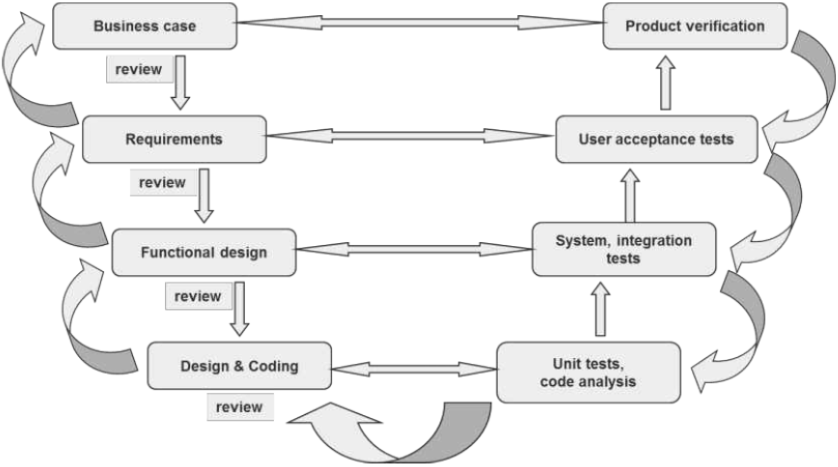
\includegraphics[width=1\textwidth]{topics/bi-wsi-si-22/images/vModel.png}
    \caption{V-model}
    \label{}
\end{figure}
\subsection{Pozitivní vs negativní testy}
\begin{itemize}
    \item funguje, co fungovat má?
    \item nefunguje, co fungovat nemá?
\end{itemize}
\subsection{Black box vs White box}
\begin{itemize}
    \item White box
    \begin{itemize}
        \item vidíme implementaci
        \item strukturální testy
    \end{itemize}
    \item Black box
    \begin{itemize}
        \item testuje se oproti rozhraní
        \item nezajímá nás implementace
        \item pohled ze strany uživatele
    \end{itemize}
\end{itemize}
\section{Detailnější rozdělení testů}
\begin{itemize}
    \item stresové testy
    \item specifické testy
    \item uživatelské testy
    \item regresní testy
\end{itemize}
\subsection{Systémové testy}
ověřují aplikaci jako funkční celek, aplikovávají se funkční i nefunkční testy.
\begin{itemize}
    \item stresové testy
    \item recovery testy
    \item bezpečnostní testy
    \item výkonostní testy
\end{itemize}
\subsection{Regresní testy}
Testy částí systému, nad kterými v aktuálním releasu neproběhli žádné změny.
Ověření, že nové změny nezkazili něco, co už fungovalo.
\subsection{Atributy testu}
\begin{itemize}
    \item Power - pravděpodobnost nalezení problému, pokud existuje
    \item Representative - odpovídá tomy, co asi uživatel nejpravděpodobněji udělá
    \item Repeatable - snadno a levně znovupoužitelné
    \item Cost - náklady, čas a pracnost
    \item Motivating - motivovanost pro opravu chyby
\end{itemize}
\subsection{Akceptační vs kvalifikační test}
\begin{itemize}
    \item kvalifikační - oveření u dodavatele, ověření zda už může být produkt předán klientovi
    \item akceptační - ověření u zákazníka, zákazník si na základě vlastních scénářů otestuje systém (jestli odpovídá požadavkům)
\end{itemize}
\section{Automatizace testů}
\begin{itemize}
    \item opakovatelnost a konzistence
    \item testy mají stejné výsledky nezávisle na počtu opakování
    \item odpadá nutnost opakovaného provádění toho stejného testu člověkem
    \item znovupouživatelnost (provádění stejných testů v různých prostředí s různou konfigurací a úpravami dat)
    \item baseline test (automatizace umožňuje velkou sadu testů)
\end{itemize}
Pro automatizace jsou obzvlášť vhodné regresní testy. Automatizace může probíhat na serveru, ale i na stroji vývojáře.
Vhodné při použití continuous integration.
\subsection{Smoke testing}
Jendá se spuštění sady testů, které testují, zda-li důležité funkce systému fungují. Používá se třeba při dělání buildů,
aby se ujistilo, že nová verze buildu bude stabilní a je možné jí dále testovat.
\end{document}